\documentclass[a4paper]{article}
\usepackage{float}
\usepackage[spanish,es-tabla]{babel}
\usepackage[T1]{fontenc}
\usepackage[spanish]{babel}
\usepackage{graphicx} 
\usepackage[utf8]{inputenc}
\usepackage{amsmath}
\usepackage{longtable}
\usepackage{graphicx}
\usepackage[colorinlistoftodos]{todonotes}
\usepackage[letterpaper,top=2.5cm,bottom=2.5cm,left=2cm,right=2cm,marginparwidth=2.5cm]{geometry}
\renewcommand{\baselinestretch}{1.25}


\title{Informe Física 3}
\author{Danny Córdova, Edwin Dávila}
\date{7 de Marzo del 2023}



\begin{document}

\maketitle

\section{Introducción}
En la presente práctica se elaboró un experimento que ayuda a calcular el valor de la gravedad a un nivel aproximado. Para el experimento se hizo uso de un tipo de movimiento dentro de la cinemática: el movimiento parabólico. Se usó una esfera pequeña de vidrio para evitar así la fricción y que los datos sean más correctos. El objetivo general de esta práctica es analizar las ecuaciones del movimiento parabólico para así poder calcular el valor de la aceleración de la gravedad.

\section{Metodología experimental}
Las unidades usadas en este experimento son las del SI. Las incertidumbres respectivas de los instrumentos de medida son:

\begin{table}[H]
    \centering
    \begin{tabular}{|c|c|}
    \hline
        Micrómetro Palmer & $\pm0,01 mm$ \\ \hline
        Regla  & $\pm 1 mm$ \\ \hline
        Metro  & $\pm 1 mm$ \\ \hline
        Cronómetro digital  & $\pm 0,01 ms$ \\ \hline
    \end{tabular}
    \caption{Incertidumbre de los instrumentos de medida}
    \label{Incertidumbre de los instrumentos de medida}
\end{table}

Se hicieron 30 medidas del movimiento parabólico y del diámetro de la esfera, aunque la medida del diámetro de la esfera tenga una incertidumbre de $\pm0,01 mm$, se tuvo que aproximar a un valor de una incertidumbre de 1mm debido a que no se podía saber si el láser del cronómetro digital iba a calcular el tiempo de paso exacto por el diámetro de la esfera.

Las variables directas que se miden en este experimento son:
\begin{enumerate}
  \item Diámetro de la esfera (d).
  \item Tiempo de obturación de la esfera por el sensor(t).
  \item Altura de la mesa (h).
  \item Distancia del movimiento en x (x).
\end{enumerate}

Las variables indirectas que se calculan a partir de la información obtenida son:
\begin{enumerate}
  \item Velocidad inicial en x($V_x$).
  \item Gravedad (g).
\end{enumerate}

Las fórmulas usadas en este experimento son:
\begin{equation}
    d=V_xt
\end{equation}
donde d es la distancia en x del movimiento parabólico, $V_x$ la velocidad inicial en x y t el tiempo.

\begin{equation}
   h=Vo_y+\frac{gt^2}{2}
\end{equation}
donde h es la altura en y, $Vo_y$ la velocidad inicial en y, g la gravedad

\begin{equation}
\Delta Z = \sqrt{{(\frac{\partial Z}{\partial A}*\Delta A)}^2+{(\frac{\partial Z}{\partial B}*\Delta B)}^2+\dots}
\end{equation}
donde $\Delta Z$ representa la propagación de incertidumbre estadística cuando se realizan varias mediciones, $\frac{\partial Z}{\partial A}$ la derivada parcial de F con respecto a A y $\Delta A$ la incertidumbre de A.

\begin{equation}
\mu= \frac{\displaystyle\sum_{i=1}^{n} x_i}{n}
\end{equation}
donde $\mu$ es la media del conjunto $x_i$ y n el número de elementos del conjunto $x_i$.

\begin{equation}
\sigma = \sqrt{\frac{1}{n-1}\displaystyle\sum_{i=1}^{n} {(x_i-\mu)}^2}
\end{equation}
donde $\sigma$ es la desviación estándar.

\begin{equation}
\varepsilon_e=\frac{\sigma}{\mu \sqrt{n}}*100\%
\end{equation}
donde $\varepsilon_e$ es el error estadístico.

\begin{equation}
e=\frac{|g_{exp}-g_{teo}|}{g_{teo}}\times 100\%
\end{equation}
donde e es el error porcentual, $g_{exp}$ la gravedad experimental y $g_{teo}$ la gravedad teórica.

\begin{equation}
y=h-\frac{gx^2}{2V_{o_x}^2}
\end{equation}
donde y es la altura en función a la distancia en x.

\section{Resultados y observaciones}

El valor promedio de los datos iniciales (ver sección de anexos) y el valor de los datos que solo se midieron una vez es:
\begin{table}[H]
\begin{center}
\begin{tabular}{| c | c |}
\hline
\multicolumn{2}{ |c| }{Medidas iniciales} \\ \hline
Diámetro de la esfera & 15,56 $\pm {1mm}$  \\ 
Altura de la mesa & 89.1 $\pm {1 mm}$\\
Tiempo de obturación & 13,11 $\pm {0,01 ms}$\\
Distancia en x & 0,501 $\pm {0,001m}$\\

\hline
\end{tabular}
\caption{Medidas iniciales}
\label{table:incertidumbre de instrumentos}
\end{center}
\end{table}

Se obtiene la velocidad instantánea a partir del tiempo en el que la esfera pasa por el sensor a través de la fórmula (1). Despejando $V_x$ obtenemos 
\[V_x=\frac{d}{t}\]

La incertidumbre de la velocidad se calcula a partir de (2):

\[\Delta V_x =\sqrt{({\frac{1}{t}(\Delta{d}))^2+  (-\frac{d}{t^2} (\Delta{t}))^2}}=0,001 m/s\]

Usando las ecuaciones (1) y (2) despejando t en (1) y reemplazándolo en (2) se obtiene la fórmula de la gravedad:

\[g=\frac{2h V_x^2 }{d^2}\]

Se calcula un valor de la gravedad para cada conjunto de datos y se saca su media a partir de (3):

\[\mu _g=\frac{\displaystyle\sum_{i=1}^{n} g_i}{n}=9,95 m/s^2\]

Se calcula el valor de la incertidumbre de la gravedad mediante (3) y se obtiene:

\[\Delta g =\sqrt{({\frac{2V_x^2}{d^2}(\Delta{h}))^2+  (\frac{4hV_x}{d^2} (\Delta{V_ox}))^2 +(-\frac{2hV_x^2}{d^3} (\Delta{d}))^2}}=0,028 m/s^2\]

Con el valor promedio se calcula la desviación estándar a partir de (5):
\[\sigma_g = \sqrt{\frac{1}{30-1}\displaystyle\sum_{i=1}^{30} {(g_i-\mu_g)}^2}=0,1528\]

El error estadístico se calcula a partir de (6):
\[ \varepsilon_e=\frac{\sigma_g}{\mu_g \sqrt{30}}*100\%= 0,2805\% \]

Por último, con el valor de la gravedad calculado por el \textit{Gravity Information System PTB} ($9.7734 m/s^2$)se calcula el error porcentual a partir de (7):
\[ \epsilon=\frac{|g_{exp}-g_{teo}|}{g_{teo}}\times100\% = 1,763\% \]

Luego de calcular estos datos, se calcula el promedio de la velocidad instantánea con (4) y se obtiene:
\[Media=\frac{\displaystyle\sum_{i=1}^{n} Vx_i}{n}=1,187 m/s\]

Debido a que la incertidumbre ya fue calculada, se obtiene que la velocidad inicial $V_{o_x}=1,187\pm {0,001} m/s$

Si se quiere conocer la posición vectorial en función del tiempo tenemos que:

\[\Vec{r(t)}=(V_{o_x}t)\Vec{i}+(h-\frac{gt^2}{2})\Vec{j}\]
Reemplazando con los datos obtenidos se tiene:
\[\Vec{r(t)}=((1,187\pm 0,001 m/s)\times t)\Vec{i}+((0.891 \pm 0,001 m)-\frac{(9.950 \pm 0,028 m/s^2) \times t^2}{2})\Vec{j}\]

Usando (8), se tiene la fórmula de la trayectoria:
\[y=0.891m-\frac{9.95m/s^2 \times x^2}{2(1,187m/s)^2}\]

Usando la herramienta digital GeoGebra, el gráfico del desplazamiento usando la fórmula de arriba es:
\begin{figure} [H]
    \centering
    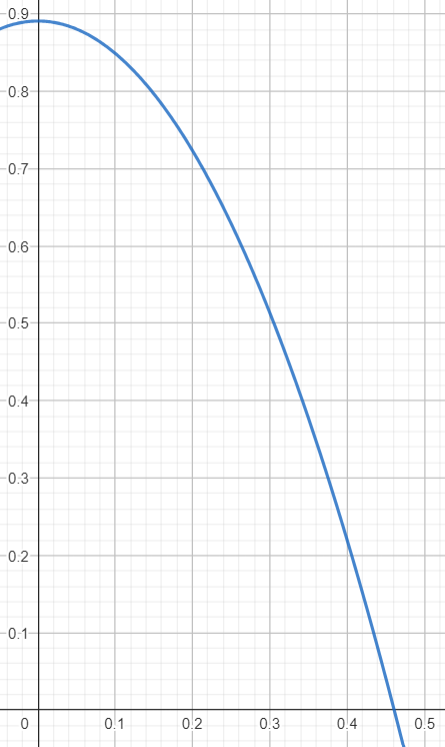
\includegraphics{Figura_Mov_Parabolico.png}
    \caption{Gráfico de la trayectoria}
    \label{Trayectoria}
\end{figure}

\section{Conclusiones}

Mediante un experimento relativamente sencillo se pudo calcular el valor de la gravedad con un nivel de error bastante bajo (solo el 1,763 \%). Este hecho demuestra que las teorías físicas se pueden confirmar o desechar con la ayuda del equipo necesario. El objetivo de esta práctica se cumplió exitosamente, se pudo modelar matemáticamente un movimiento que se observa a diario, se confirmaron las leyes de la cinemática experimentalmente para el movimiento parabólico y las predicciones concuerdan con los resultados obtenidos en la realidad. 

\section{Anexos}

\begin{table}[H]
\begin{center}
\begin{tabular}{| c | c |}
\hline
\multicolumn{2}{ |c| }{Diámetro de la esfera (mm)} \\ \hline
        15,43  $\pm {0,01}$ & 15,61 $\pm {0,01}$ \\ \hline
        15,44  $\pm {0,01}$& 15,61$\pm {0,01}$  \\ \hline
        15,45  $\pm {0,01}$& 15,60$\pm {0,01}$  \\ \hline
        15,52  $\pm {0,01}$& 15,59$\pm {0,01}$  \\ \hline
        15,53  $\pm {0,01}$& 15,56$\pm {0,01}$  \\ \hline
        15,53  $\pm {0,01}$& 15,54$\pm {0,01}$  \\ \hline
        15,51  $\pm {0,01}$& 15,57 $\pm {0,01}$ \\ \hline
        15,50  $\pm {0,01}$& 15,63$\pm {0,01}$  \\ \hline
        15,60  $\pm {0,01}$& 15,68$\pm {0,01}$  \\ \hline
        15,58  $\pm {0,01}$& 15,64$\pm {0,01}$  \\ \hline
\end{tabular}
\caption{Diámetro de la esfera medida 20 veces.}
\label{tab:diámetro de la esfera}
\end{center}
\end{table}

\begin{table}[H]
    \centering
    \begin{tabular}{|l|l|}
    \hline
        Tiempo de paso (ms)  & Distancia en x (m)  \\ \hline
        12,93  & 0,503  \\ \hline
        13,25  & 0,497  \\ \hline
        13,12  & 0,494  \\ \hline
        12,99  & 0,502  \\ \hline
        13,01  & 0,503  \\ \hline
        13,14  & 0,504  \\ \hline
        12,77  & 0,51  \\ \hline
        13,14  & 0,498  \\ \hline
        13,29  & 0,5  \\ \hline
        13,1  & 0,5  \\ \hline
        13,3  & 0,499  \\ \hline
        13,08  & 0,503  \\ \hline
        13,3  & 0,499  \\ \hline
        13,18  & 0,5  \\ \hline
        13,14  & 0,498  \\ \hline
        12,94  & 0,502  \\ \hline
        13,29  & 0,497  \\ \hline
        13,09  & 0,498  \\ \hline
        12,95  & 0,5  \\ \hline
        13,08  & 0,503  \\ \hline
        13,01  & 0,504  \\ \hline
        12,86  & 0,508  \\ \hline
        13,11  & 0,502  \\ \hline
        13,18  & 0,501  \\ \hline
        13,14  & 0,498  \\ \hline
        13,27  & 0,5  \\ \hline
        12,98  & 0,502  \\ \hline
        13,3  & 0,5  \\ \hline
        13,14  & 0,497  \\ \hline
        13,09  & 0,502  \\ \hline
    \end{tabular}
\end{table}



\begin{table}[H]
    \centering
    \begin{tabular}{|l|l|}
    \hline
        Velocidad instantánea $V_x$ (m/s)  & Gravedad estimada ($m/s^2$)  \\ \hline
        1,203  & 10,13  \\ \hline
        1,174  & 9,877  \\ \hline
        1,186  & 10,20  \\ \hline
        1,198  & 10,07  \\ \hline
        1,196  & 10,00  \\ \hline
        1,184  & 9,766  \\ \hline
        1,218  & 10,10  \\ \hline
        1,184  & 10,00  \\ \hline
        1,171  & 9,700  \\ \hline
        1,187  & 9,984  \\ \hline
        1,170  & 9,724  \\ \hline
        1,189  & 9,895  \\ \hline
        1,170  & 9,724  \\ \hline
        1,180  & 9,863  \\ \hline
        1,184  & 10,00  \\ \hline
        1,202  & 10,15  \\ \hline
        1,171  & 9,818  \\ \hline
        1,188  & 10,08  \\ \hline
        1,201  & 10,22  \\ \hline
        1,189  & 9,895  \\ \hline
        1,196  & 9,962  \\ \hline
        1,210  & 10,04  \\ \hline
        1,187  & 9,889  \\ \hline
        1,180  & 9,823  \\ \hline
        1,184  & 10,00  \\ \hline
        1,172  & 9,729  \\ \hline
        1,198  & 10,09  \\ \hline
        1,170  & 9,686  \\ \hline
        1,184  & 10,04  \\ \hline
        1,188  & 9,919  \\ \hline
        \end{tabular}
\end{table}

Si se desea saber el valor promedio de los datos medidos solo se usa la ecuación (3). 

\end{document}
